\documentclass[letterpaper, 11pt]{article}
\usepackage{hyperref}
\usepackage{graphicx}
\usepackage{caption}
\usepackage{subcaption}
\usepackage{amsmath}
\usepackage{tikz}
\renewcommand{\baselinestretch}{1.1}
\usepackage[margin=1.2in]{geometry}
\usepackage{xcolor}
\hypersetup{
    colorlinks,
    linkcolor={red!50!black},
    citecolor={blue!50!black},
    urlcolor={blue!80!black}
}

\begin{document}
\title{WebPlotDigitizer Theory}
\author{Ankit Rohatgi\footnote{E-Mail: ankitrohatgi@hotmail.com}}
\maketitle
\tableofcontents
\newpage

\section{Axes Calibration}

\subsection{XY Axes}

\begin{figure}[h]
\centering
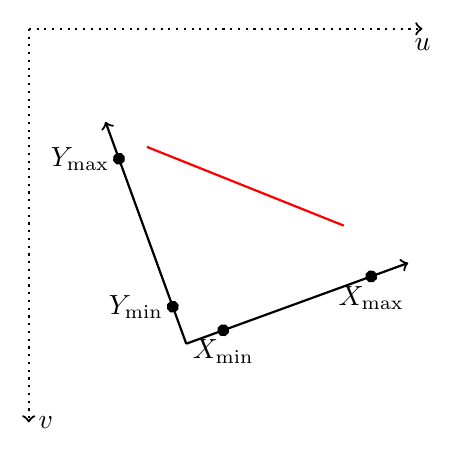
\begin{tikzpicture}
\draw[thick,dotted,->] (0,5) -- (0,0);
\draw[thick,dotted,->] (0,5) -- (5,5);
\draw[rotate around={20:(2,1)},thick,->] (2,1) -- (5,1);
\draw[rotate around={20:(2,1)},thick,->] (2,1) -- (2,4);
\draw[red,thick,-] (1.5,3.5) -- (4,2.5);
\filldraw[rotate around={20:(2,1)},black] (2.5,1) circle (2pt) node[anchor=north]{$X_{\min}$};
\filldraw[rotate around={20:(2,1)},black] (4.5,1) circle (2pt) node[anchor=north]{$X_{\max}$};
\filldraw[rotate around={20:(2,1)},black] (2,1.5) circle (2pt) node[anchor=east]{$Y_{\min}$};
\filldraw[rotate around={20:(2,1)},black] (2,3.5) circle (2pt) node[anchor=east]{$Y_{\max}$};
\draw (0,0) node[anchor=west]{$v$};
\draw (5,5) node[anchor=north]{$u$};

\end{tikzpicture}
\caption{Four points on the axes help compute the affine transformation needed to map the data in $(x,y)$ coordinates to the pixels $(u,v)$ on the screen.}
\end{figure}

% notation:
% (u,v) - pixels
% (x_i, y_i) - data

\begin{equation}
\begin{bmatrix}
x \\
y 
\end{bmatrix}
= 
\begin{bmatrix}
a_1 & a_2 \\
a_3 & a_4
\end{bmatrix}
\begin{bmatrix}
u \\
v
\end{bmatrix}
+
\begin{bmatrix}
c_0 \\
c_1
\end{bmatrix}
\end{equation}

\begin{equation}
\begin{bmatrix}
a_1 & a_2\\
a_3 & a_4
\end{bmatrix}
=
\begin{bmatrix}
x_{\max} - x_{\min} & 0 \\
0 & y_{\max} - y_{\min}
\end{bmatrix}
\begin{bmatrix}
u_1 - u_0 & u_3 - u_2\\
v_1 - v_0 & v_3 - v_2
\end{bmatrix}^{-1}
\end{equation}


% x_min = a1*u_0 + a2*v_0 + c_0
% y_min = a3*u_2 + a4*v_2 + c_1
\begin{equation}
\begin{bmatrix}
c_0 \\
c_1
\end{bmatrix}
=
\begin{bmatrix}
x_{\min} \\
y_{\min}
\end{bmatrix}
-
\begin{bmatrix}
a_1 u_0 + a_2 v_0 \\
a_3 u_2 + a_4 v_2
\end{bmatrix}
\end{equation}

TODO: add note about handling log scale, dates etc.

\subsection{Bar Axes}

\begin{figure}[h!]
\centering
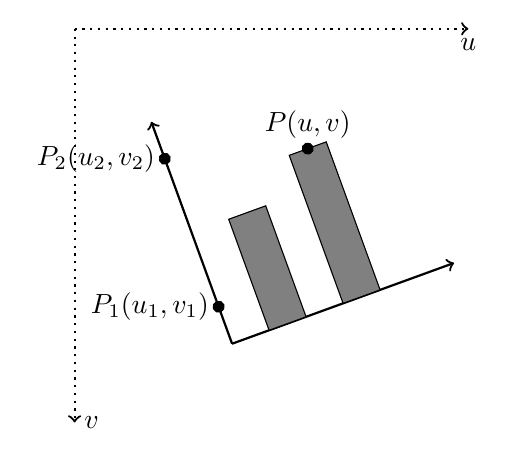
\begin{tikzpicture}
\draw[thick,dotted,->] (0,5) -- (0,0);
\draw[thick,dotted,->] (0,5) -- (5,5);
\draw[rotate around={20:(2,1)},thick,->] (2,1) -- (5,1);
\draw[rotate around={20:(2,1)},thick,->] (2,1) -- (2,4);

\filldraw [rotate around={20:(2,1)},fill=gray, draw=black] (2.5,1) rectangle (3,2.5);
\filldraw [rotate around={20:(2,1)},fill=gray, draw=black] (3.5,1) rectangle (4,3);

\filldraw[rotate around={20:(2,1)},black] (2,1.5) circle (2pt) node[anchor=east]{$P_1 (u_1, v_1)$};
\filldraw[rotate around={20:(2,1)},black] (2,3.5) circle (2pt) node[anchor=east]{$P_2 (u_2, v_2)$};
\filldraw[rotate around={20:(2,1)},black] (3.75,3) circle (2pt) node[anchor=south]{$P (u, v)$};
\draw (0,0) node[anchor=west]{$v$};
\draw (5,5) node[anchor=north]{$u$};

\end{tikzpicture}
\caption{Two points on the axes}
\end{figure}

\begin{equation}
\vec v_{12} = (u_2-u_1)\hat i + (v_2 - v_1) \hat j
\end{equation}

\begin{equation}
\vec v_p = (u-u_1)\hat i + (v - v_1) \hat j
\end{equation}

projected distance along the axis
\begin{equation}
d_p = \frac{\vec v_p \cdot \vec v_{12}}{|| \vec v_{12} ||}
\end{equation}

\begin{equation}
y = (y_2 - y_1) \frac{d_p}{d_{12}} + y_1 \\
\end{equation}
\begin{equation}
y = \left\{\frac{(u - u_1)(u_2 - u_1) + (v - v_1)(v_2 - v_1)}{(u_2 - u_1)^2 + (v_2 - v_1)^2}\right\}(y_2 - y_2) + y_1
\end{equation}

\subsection{Polar Axes}
\subsection{Ternary Diagram}
\subsection{Circular Chart Recorder}

\section{Curve Extraction Algorithms}

\subsection{Averaging Window}
\subsection{X Step with Interpolation}
\subsection{X Step}
\subsection{Bar Extraction}

\section{Measurements}

\end{document}